\documentclass[a4paper,12pt]{article}
\usepackage[spanish]{babel}
\hyphenation{co-rres-pon-dien-te}
\usepackage[utf8]{inputenc}
\usepackage[T1]{fontenc}
\usepackage{graphicx}
\usepackage[pdftex,colorlinks=true, pdfstartview=FitH, linkcolor=blue,
citecolor=blue, urlcolor=blue, pdfpagemode=UseOutlines, pdfauthor={H. Asorey},
pdftitle={F3B+F4B - Guía 03}]{hyperref}
\usepackage[adobe-utopia]{mathdesign}

\hoffset -1.23cm
\textwidth 16.5cm
\voffset -3.5cm
\textheight 26.5cm

%----------------------------------------------------------------
\begin{document}
\title{
{\normalsize{Universidad Nacional de Río Negro - Profesorado de Física}}\\
Física 3B+4A  2018 \\ Guía 04: Máquinas térmicas
}
\author{Asorey}
\date{03 de Mayo de 2018} 
\maketitle

\begin{enumerate}
	\setcounter{enumi}{28}      %% esta guia va del problema 29 al XX

	\item {\bf{Carnot, con números}}

		Una máquina térmica opera siguiendo un ciclo de Carnot erogando una
		potencia de $3$\,MW con un rendimiento del 75\%.  Contiene $100$\,moles de
		un gas ideal triatómico, y está instalada cerca de un río a temperatura
		$T_C=280$\,K. La puesta en marcha se realiza calentando al gas desde
		CNPT en forma isocórica hasta alcanzar la temperatura de trabajo.
		\begin{enumerate}
			\item Dibuje el ciclo en un diagrama P-V.
			\item Complete el cuadro de estados y el cuadro de transformaciones.
		\end{enumerate}
		{\bf{R}}: 
	
	\item {\bf{Máquina de Carnot directa y reversa}}
		
		Suponga una máquina térmica que funciona mediante un ciclo de Carnot
		entre dos fuentes a temperaturas $T_A=700$\,K y $T_C=300$\,K y utiliza
		como fluido un gas ideal di-atómico. Al iniciar el ciclo, el gas se
		encuentra a la temperatura $T_A$, una presión de $10$\,hPa y ocupa un
		volumen de $0.007$\,m$^3$. Al finalizar el primer tramo del ciclo la
		presión del gas desciende a $P_B=8$\,hPa.
		\begin{enumerate}
			\item Dibuje el ciclo en un diagrama P-V.
			\item Complete el cuadro de estados y el cuadro de transformaciones
			\item Halle el rendimiento total el ciclo, y compruebe si coincide
				con el valor esperado para un ciclo de Carnot.
			\item ¿Dependerá el rendimiento de la atomicidad del gas? ¿y la
				cantidad total de trabajo obtenida?
			\item Calcule la potencia entregada por la máquina sabiendo que la
				misma puede funcionar a 210 ciclos por segundo.
			\item Invierta el ciclo y calcule el trabajo que es necesario
				entregar a la máquina térmica para hacerla funcionar en el
				sentido inverso.
		\end{enumerate}
		{\bf{R}}: 
	
	\item {\bf{Auto 1: rendimiento}}\label{auto1}
		
		Para alcanzar una velocidad máxima de 150\,km/h se requiere toda la
		potencia de un motor de automóvil de 100\,kW. ¿Cuánta nafta se requiere
		para recorrer 100\,km cuando el motor tiene un eficiencia de 25\%?
		Discutir el balance energético total. Equivalente energético de la
		nafta: 12 kWh/kg.
		\\{\bf{R}}: 
	
	\item {\bf{Energía del mar}}
		
		Se quiere usar la diferencia de temperatura entre la superficie del
		agua de mar de 25\,$^\mathrm{o}$C y de las capas profundas de
		4\,$\mathrm{o}$C para producir energía eléctrica.
		\begin{enumerate}
			\item ¿Cuál es la eficiencia termodinámica máxima que esperaría
				encontrar con este método de producción de energía?
			\item ¿Cuántos m$^3$ de agua por segundo se necesitaría para
				producir 1 GW de trabajo neto (eléctrico)?
		\end{enumerate}
		{\bf{R}}: 
	
	\item {\bf{Horno solar}}
		
		Un diseño de horno solar permite calentar agua hasta
		90$^\mathrm{o}$\,C. Una persona propone usar esta agua caliente para
		hacer funcionar una máquina térmica. ¿Qué eficiencia se podría alcanzar
		para esa máquina si la temperatura ambiente es de 20$^\mathrm{o}$\,C?
		Si la constante solar es de $1400$\,W\,m$^2$ y la absorción atmosférica
		en nuestras latitudes es del $50\%$, ¿cuál es el área que debe tener el
		colector solar para calentar $1$\,kg de agua desde temperatura ambiente
		hasta la temperatura máxima en $1$\,minuto?
		\\{\bf{R}}: 
	
	\item {\bf{Máquina térmica}}
		
		Una máquina térmica tiene una eficiencia del 30\% y eroga $3$\,GW de
		potencia mecánica.
		\begin{enumerate}
			\item ¿Qué cantidad de calor recibe de la fuente caliente? ¿Qué
				cantidad de calor entrega al medio ambiente?
			\item Éste calor debe ser entregado a un río cuya temperatura no
				debe subir más de 2$^\mathrm{o}$\,C. ¿Qué caudal mínimo (en
				m$^3$ s$^{-1}$) debe tener ese río?
		\end{enumerate}
		{\bf{R}}: 
	
	\item {\bf{Trigo}}
		
		El valor nutritivo del trigo que se produce en un metro cuadrado de
		tierra fértil es de $2$\,kWh. Si en esa región agrícola la irradiancia solar
		durante el verano es $\sim 700$\,W\,m$^{-2}$ durante unas 7 horas
		diarias en promedio y que el trigo demora cinco meses en madurar.  
		¿Cual es el rendimiento energético del trigo? 
		\\{\bf{R}}:

	\item {\bf{Auto 2: ciclo Otto}}
		
		El ciclo Otto opera en los motores de autos que funcionan con nafta
		(gasolina) como combustible. Es usual hablar del ciclo de cuatro etapas
		(Admisión, Compresión, Explosión y Escape), aunque en realidad son seis
		las etapas que experimenta la mezcla de combustible y aire: 1)
		expansión de la mezcla a presión constante (admisión, $n$ aumenta); 2)
		compresión adiabática (compresión); 3) calentamiento isócoro
		(combustión); 4) expansión adiabática (explosión+expansión); 5)
		enfriamiento isócoro; 6) compresión isóbara (escape, $n$ disminuye).
		Descartando las etapas 1 y 6, donde hay cambio en la cantidad de gas,
		suponiendo que durante las etapas 2, 3, 4 y 5 la cantidad de mezcla es
		$n=0.02$\,mol (valor aproximado para un motor de $2000$\,cm$^3$), y
		utilizando los valores del diagrama PV visto en clase (página 17/30
		Clase U02C06), realice los siguientes ejercicios:  
		\begin{enumerate}
			\item Complete el cuadro de estados $A$, $B$, $C$ y $D$. 
			\item Complete el cuadro de las transformaciones $2$, $3$, $4$ y
				$5$.  
			\item El rendimiento termodinámico del motor. Compárelo con el
				rendimiento de un ciclo de Carnot equivalente y con el obtenido
				en el problema \ref{auto1}.
			\item Si el motor funciona en régimen a $3600$\,RPM, calcule la
				cantidad de calor producida por el consumo de combustible, el
				trabajo neto liberado y la cantidad de calor liberada en la
				atmósfera cada hora de funcionamiento.		
		\end{enumerate}
		{\bf{R}}: 

	\item {\bf{Ciclo combinado en el océano}} 
		
		Tres máquinas térmicas idénticas que funcionan con un ciclo de Carnot
		se conectan en una configuración de ciclo combinado, de forma tal que
		el calor no aprovechado por una de las máquinas es utilizado por la
		siguiente máquina del complejo.  El rendimiento de cada etapa debe ser
		$\eta_i=0.6$. La fuente fría de la última de las máquinas es el océano
		Atlántico, cuya temperatura es $T_f=276$\,K. Si la última etapa del
		ciclo eroga $1$\,GW de potencia, haga un esquema de la situación
		planteada y responda lo siguiente:
		\begin{enumerate} 
			\item La cantidad total de calor entregada al océano en una hora de
				funcionamiento.
			\item La cantidad de calor que cada hora suministra la fuente
				caliente en la primera etapa.
			\item El trabajo neto entregado por cada etapa del ciclo y el
				trabajo neto total.
			\item Las dos temperaturas de trabajo de cada una de las máquinas.
			\item El rendimiento global, y la potencia útil total erogada por
				el complejo.
		\end{enumerate}
		{\bf{R}}: 
	
	\item {\bf{Máquinas en cascada}}
		
		Una instalación de ciclo combinado dispone de dos máquinas térmicas
		$M_A$ y $M_B$ conectadas en cascada, es decir, el calor $Q_i$ que sale
		de la máquina $A$ es usado para generar un trabajo adicional en la
		máquina $B$.  La fuente caliente principal es una caldera de vapor
		operando a una temperatura $T_1=1000$\,K, que entrega $Q_1=500$\,MJ de
		calor. El calor residual $Q_2$ que sale de la máquina $B$ se utiliza
		para calefaccionar las oficinas de la planta, calentando agua a
		temperatura ambiente $T_i=T_2=293$\,K hasta $T_c=353$\,K.
		\begin{figure}[hhhhhb!]
			\centering
			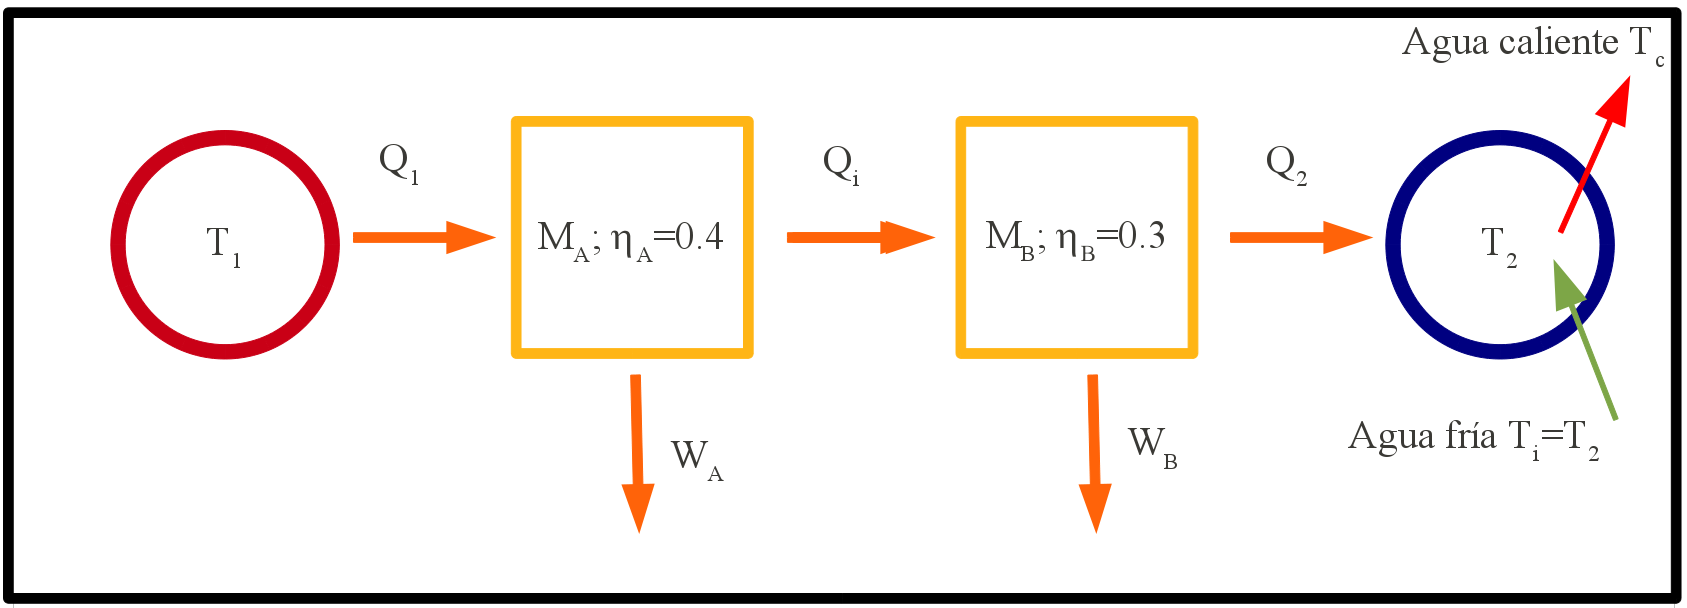
\includegraphics[width=0.6\textwidth]{maq2}
		\end{figure}
		\begin{enumerate}
			\item Calcule la cantidad de calor $Q_i$ que pasa de la máquina $A$
				a la $B$ cada segundo.
			\item Calcule el trabajo total producido:
					$W=W_A+W_B$ por segundo.
			\item Calcule la cantidad de calor $Q_2$ que pasa de la máquina $B$
				a la calefacción.
			\item Calcule el rendimiento total de la instalación de ciclo
				combinado, y diga cual es la ventaja de estas instalaciones.
			\item Compare el rendimiento anterior con el rendimiento de una
				máquina de Carnot operando entre esas temperaturas.
			\item Calcule cuantos litros de agua por segundo será posible
				calentar desde $T_2$ hasta $T_c$.
		\end{enumerate}
		{\bf{R}}: 
\end{enumerate}
\end{document}
%%%%
